\section{Introduction} \label{sec:intro}
The Vera C. Rubin Observatory is located at Cerro Pachón in the Atacama Desert in Chile. It was selected after careful consideration of various sites worldwide based on their meteorological conditions. The observatory will operate the 8.4-meter Simonyi Research Telescope, which has the capability to scan the entire southern sky in approximately three nights and is expected to start operations in 2024. Additionally, the observatory houses the LSST Camera, the largest camera ever built, with a 3.2 gigapixel resolution for the entire focal plane. The LSST Camera has a diameter of 64 cm, covering a 9.6 deg$^2$ field of view, and a plate scale of 0.2 '' pixel$^{-1}$ \citep{2009arXiv0912.0201L}.

\vspace{3mm}
The observatory is named in honor of the renowned astronomer Vera Rubin \citep{NSF_2020}, who, in 1970, pioneered the measurement of the rotation curves of disk galaxies \citep{rubin2011interesting}. Her groundbreaking work revealed that there must be more mass than what is observed in galaxies in order for stars to rotate at the observed rate without breaking apart. This additional mass is now known as dark matter, and studying it is one of the scientific goals of the Vera C. Rubin Observatory.

\vspace{3mm}
Vera Rubin received numerous awards for her contributions to astronomy, including the National Medal of Science, and even has a ridge on Mars named after her \citep{koren_2020}. In addition, she was a staunch advocate for recognizing the work of women in science and her students \citep{rubin2011interesting}.

\subsection{LSST Scientific Goals}

The Legacy Survey of Space and Time (formerly Large Synoptic Survey Telescope, LSST) has four primary scientific objectives \citep{2009arXiv0912.0201L, ivezic2019lsst}:

\begin{itemize}
    \item Inventory of the Solar System: The LSST aims to study minor bodies in the solar system, including Trans-Neptunian Objects (TNOs), asteroids, and comets, to better understand planetary formation and evolution. By analyzing their orbital elements and sizes, the LSST will provide valuable insights into the history of these objects. Additionally, studying the interaction of objects in the Main Asteroid Belt, located between Mars and Jupiter, could shed light on the origin of Near-Earth Objects (NEOs) that come from the Main Belt and enter Earth's orbit.

    \item Mapping the Milky Way: This objective involves studying the structure, dynamics, and chemical composition of stars in our galaxy, the Milky Way, to understand its formation and evolution. The LSST will also characterize stars in the solar neighborhood within 300 parsecs.

    \item Exploring the Transient Optical Sky: The LSST will conduct time-domain science to observe transient and variable phenomena such as supernovae, variable stars, and Active Galactic Nuclei (AGN). The goal is to detect and study transient and distant objects, which requires observing a large portion of the sky to increase the probability of capturing such events, obtaining high-quality images to discern differences between images, capturing data with good sampling time to detect various types of variable stars, obtaining accurate color information for classification, conducting long-term persistent observations to track the events, and processing, classifying, and rapidly publishing data for the community to enable further studies such as spectroscopy.

    \item Probing Dark Energy and Dark Matter: Dark energy, which affects the expansion of the universe, and dark matter, which accumulates mass, can be studied using various mechanisms. The LSST will utilize techniques such as weak gravitational lensing, the study of large-scale structures like galaxy clusters, Baryonic Acoustic Oscillations (BAO), and Supernova systems, among others, to probe dark energy. For the study of dark matter, the LSST will explore weak and strong lensing of galaxy mass distributions, among other approaches.

\end{itemize}

\subsection{CCD Type in LSST Camera}

The LSSTCam utilizes \textit{thick fully depleted} and back-illuminated CCDs \citep{2009arXiv0912.0201L}. These CCDs are known for their excellent response in the near-infrared regions \citep{lage2017measurements}, making them suitable for observing distant objects that are reddened by the universe's expansion. However, due to their thickness, they can exhibit effects caused by the long path that electrons must travel to the charge storage well.

\vspace{3mm}
Highly segmented, the LSSTCam can be read out completely in 2 seconds, reducing the readout noise associated with high readout speeds \citep{2009arXiv0912.0201L}. It consists of a mosaic of 205 CCDs organized into 21 science modules, each containing nine CCDs, along with four specialized corner modules for telescope guidance and alignment through active optics \citep{snyder2020laboratory}. The CCDs in the mosaic are sourced from two vendors: Imaging Technology Laboratories (ITL) and Teledyne e2v (E2V), with each CCD divided into 16 segments. Figure \ref{fig:FP_LSSTCam} illustrates the ITL detectors in greenish blue, the E2V detectors in yellow, which are used for science, and the guidance CCDs in purple.

\vspace{3mm}
As mentioned by \cite{walter2015brighter}, precise measurements of the point spread function (PSF) of galaxies are essential for the LSST's science objective in weak lensing, where the goal is to study how the shape of galaxies is modified by observing a wide field. To achieve this, it is crucial to quantify the brighter-fatter (BF) effect, which causes deformation of the PSF and is more significant in brighter objects, gradually decreasing in fainter objects \citep{lage2017measurements}. Additionally, \cite{walter2015brighter} notes that the sensors also experience an edge effect, where electrons near the edge of the sensor feel a force that pushes them inward, primarily affecting astrometry.


\begin{figure}[!htb]
    \centering
    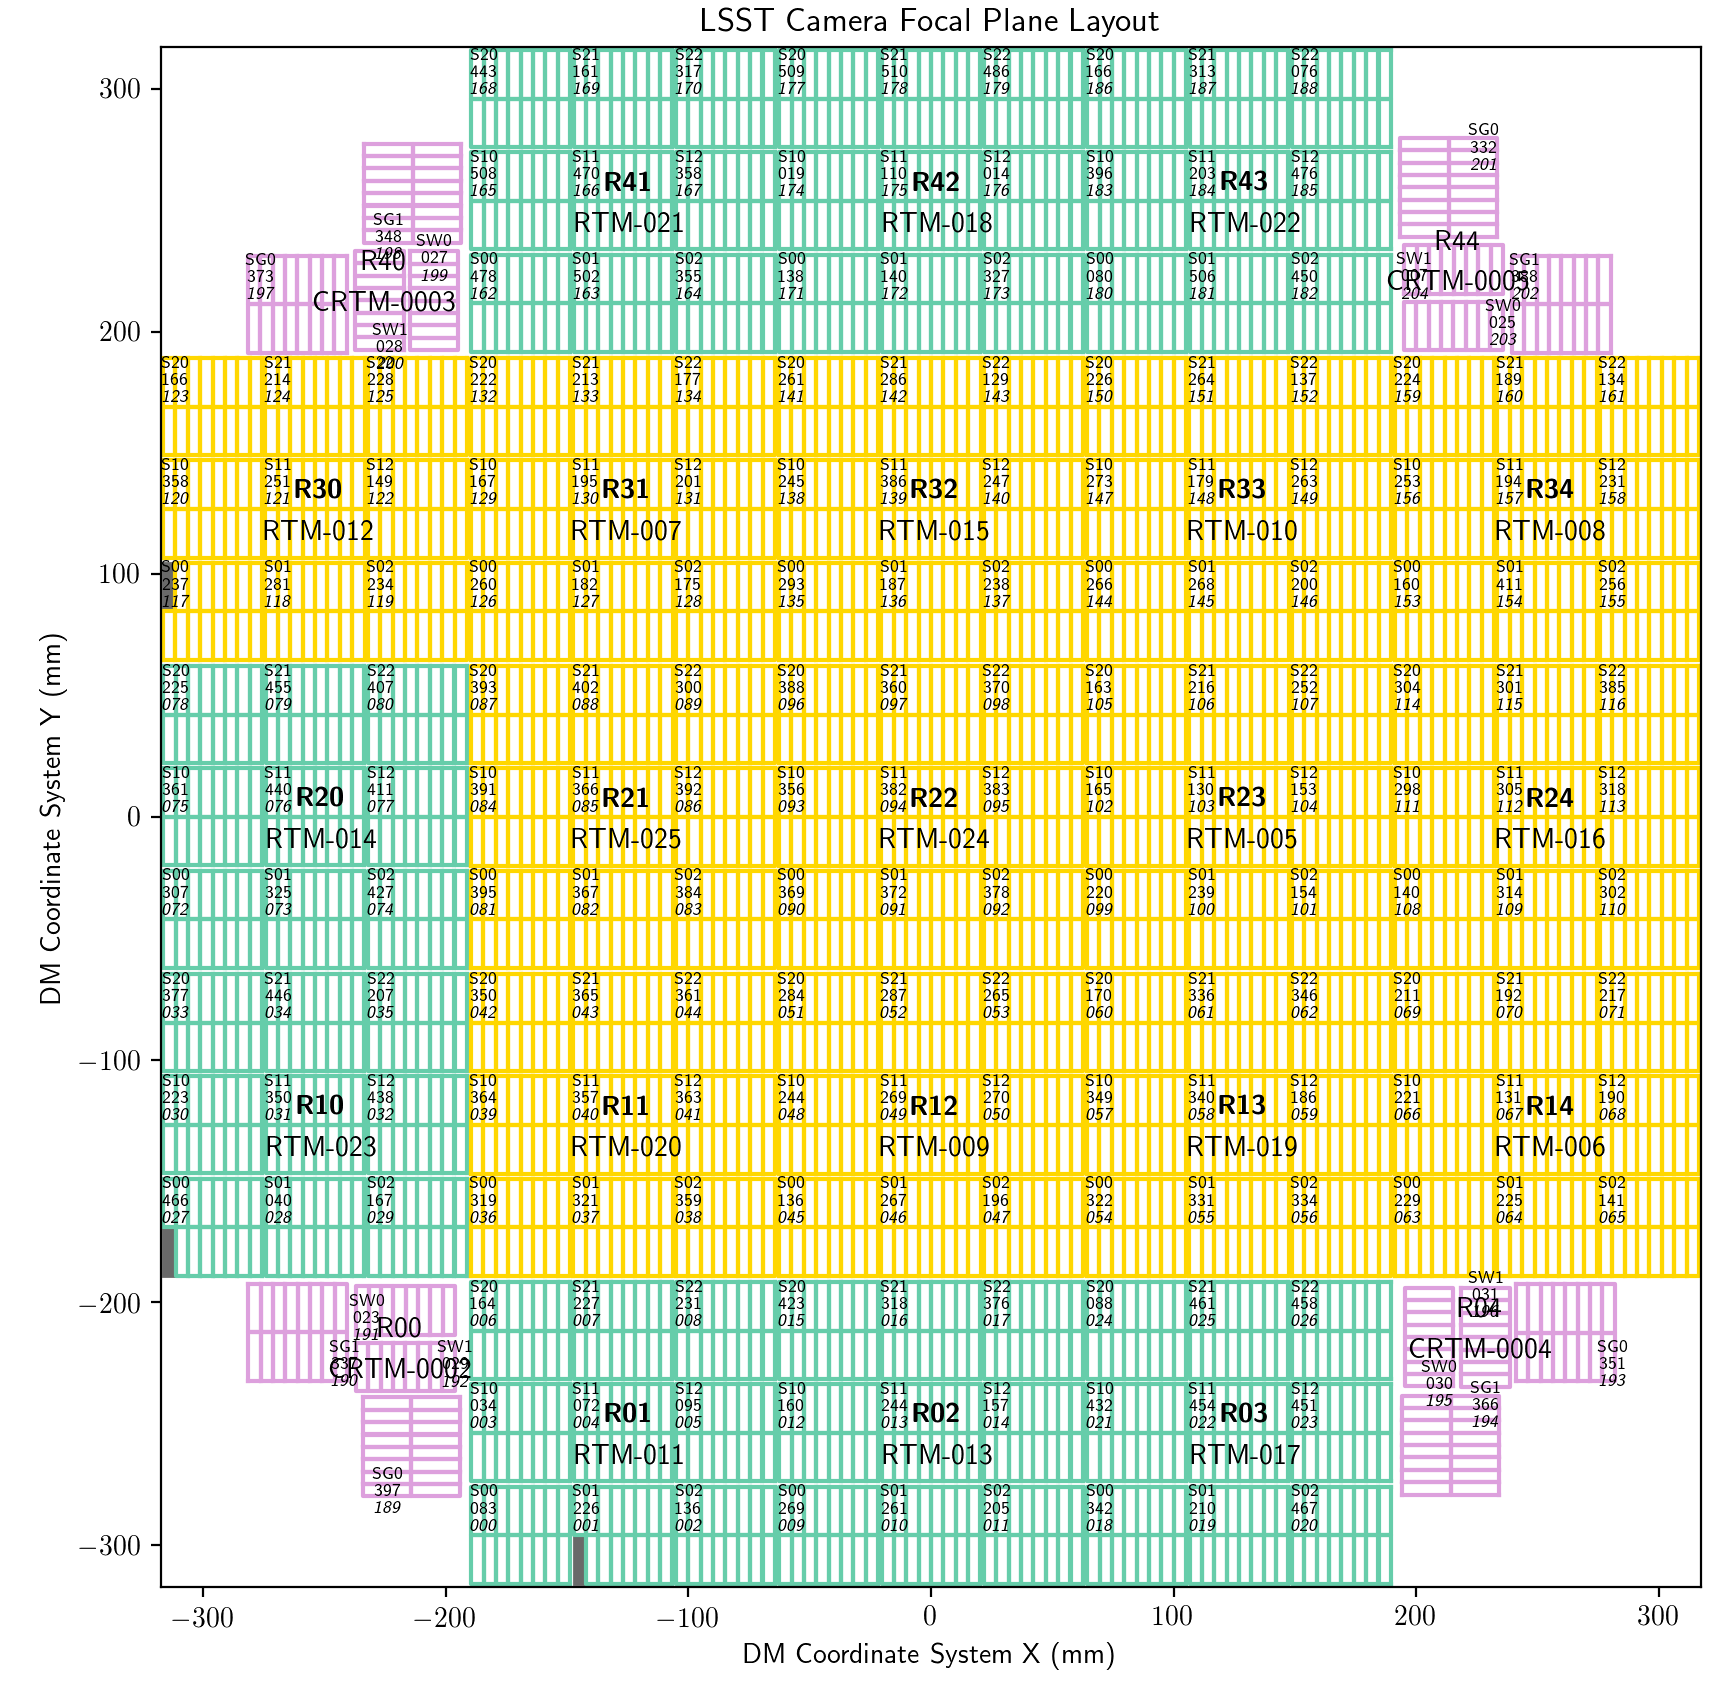
\includegraphics[width=\textwidth]{Figures/FP_layout_DM.png}
    \caption{The focal plane of the LSST camera. The vendor's CCDs' location is blue for ITL and yellow for E2V. Each CCD (a small square) is composed of 16 segments, each with its amplifier, and 189 CCDs are responsible for taking the science data. The CCDs at the corners are for focusing and synchronization with the Earth's rotation (see \href{https://www6.slac.stanford.edu/news/2020-09-08-sensors-world-largest-digital-camera-snap-first-3200-megapixel-images-slac.aspx}{LSST-SLACLab}). \textit{Image credits: Seth Digel/LSST Camera project.}}
    \label{fig:FP_LSSTCam}
\end{figure}

\subsection{What is Photon Transfer Curve (PTC)?}
The Photon Transfer Curve (PTC) is a characterization tool used to determine the fundamental parameters of a CCD, such as the gain, which represents the relationship between the electrons recorded by each pixel and their conversion to Analog-to-Digital Unit (ADU). The PTC also measures the nonlinearity of the camera and its Full Well Capacity (FWC). The gain is a crucial parameter as it impacts other vital parameters like read noise, quantum efficiency, dark current, and more, making it essential for a comprehensive understanding of CCD performance \citep{downing2006ccd}.

Figure \ref{fig:PTC} shows the PTC of segment C06 of sensor 22 of the LSSTCam. It is evident that at low fluxes, the variance is low and increases with the flux, but not linearly, until reaching the saturation point or FWC, which is $83000$ ADU for this detector. Beyond this point, the variance begins to decrease, indicating that the flux stored in each pixel of this amplifier starts to homogenize. This nonlinear behavior is exhibited by \textit{thick fully-depleted CCDs} as explained by \cite{downing2006ccd}, where charge storage in a pixel is the main cause for the deviation from the expected relationship between variance and mean number of counts in a pixel, especially in flat images \citep{walter2015brighter}. The effective area of the pixel changes with the amount of charge, decreasing as the charge accumulated in the pixel increases. As a result, very bright sources are mainly affected by this phenomenon known as the BF effect. If the pixels of the CCD segment were independent, they could be described by Poisson statistics, and the PTC would follow the green line in the figure.

\begin{figure}[!htb]
    \centering
    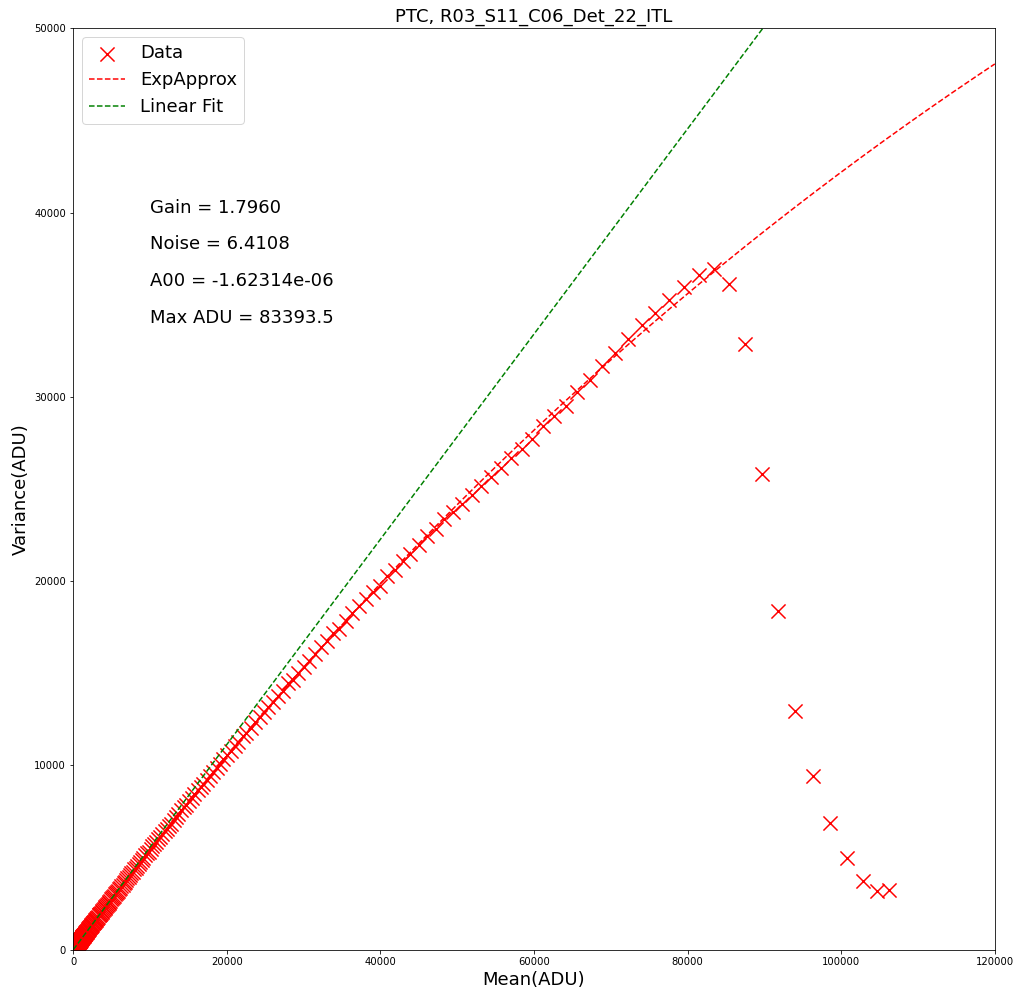
\includegraphics[width=0.7\textwidth]{Figures/PTC_R03_S11_C06_Det22.png}
    \caption{Photon Transfer Curve (PTC) for detector 22, which is located in raft 03, sensor 11, and amplifier C06, and manufactured by ITL. The red crosses represent the data points, the red line shows the EXPAPPROXIMATION fit, and the green line represents the linear fit. This PTC curve was generated using the results obtained via the \textit{DM stack}.}
    \label{fig:PTC}
\end{figure}

\subsubsection{Brigther father effect}

As mentioned previously, the charge stored in a pixel can alter the effective area of the pixel, reducing the probability that the pixel will continue to store the charge. This can result in horizontal deflection of the electrons, causing more elliptical images. This phenomenon breaks down the initial assumption of Poisson statistics and independent charge storage in each pixel, thereby modifying the relationship between the variance and the mean number of counts per pixel \citep{walter2015brighter}. This effect can impact the Point Spread Function (PSF) and may pose a potential problem for surveys that are interested in studying variations in brightness and shape of objects \citep{coulton2018exploring}.

\vspace{6mm}
This work was conducted during the RECA (Red de Estudiantes Colombiana de Astronomía) internship program in 2022\footnote{The RECA internship program is a scientific research training program in Astronomy, Astrophysics, and Cosmology for students from Colombian institutions. Program website: \href{https://recastronomia.github.io/internship/}{https://recastronomia.github.io/internship/}}. The program spanned three months and also involved other activities such as remote astronomical observations at the Teide Observatory\footnote{\href{https://www.iac.es/es/observatorios-de-canarias/observatorio-del-teide}{https://www.iac.es/es/observatorios-de-canarias/observatorio-del-teide}}.

In this report, we present the data used in Section \ref{sec:data}, describe the methodology in Section \ref{sec:methods}, present the results and analysis in Section \ref{sec:results}, and provide conclusions in Section \ref{sec:conclusions}."
